% !TeX root = e4-tp2-ej2
\documentclass[e4-tp2-main.tex]{subfiles}

\begin{document}

\section{Convertidor boost para l\'ampara LED de potencia}

\subsection{Efectos de temperatura en los LEDs}

\begin{wrapfigure}[15]{L}{0.50\textwidth}
    \centering
    \begin{subfigure}[t]{0.24\textwidth}
    	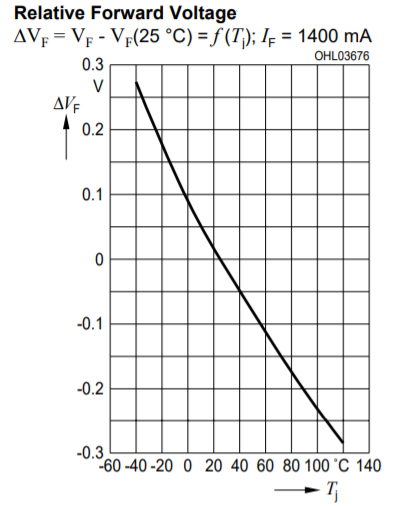
\includegraphics[width=\textwidth]{images/ej2/Cambio_Vf_LED.png}
    	\caption{Cambios en $V_f$}
    \end{subfigure}
    \begin{subfigure}[t]{0.24\textwidth}
    	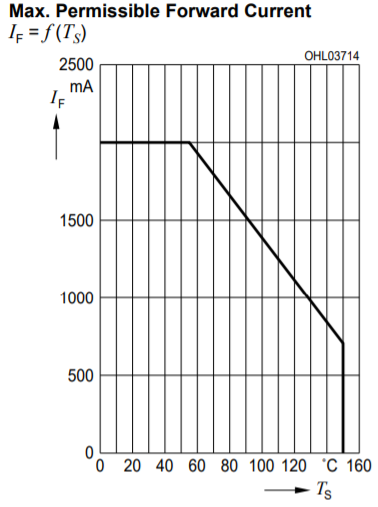
\includegraphics[width=\textwidth]{images/ej2/Cambio_If_LED.png}
    	\caption{Cambios en $I_{f_{MAX}}$}
    \end{subfigure}
    \caption{Efectos de la temperatura en los LEDs}
    \label{fig:Efec_Leds}
\end{wrapfigure}

Se utilizaron los LEDs OSRAM LUW-W5AP, los cuales a medida que aumenta su temperatura se producen variaciones de la tensión de forward ($V_f$) y la máxima corriente de forward soportada ($I_{f_{MAX}}$). Donde ante un aumento de la temperatura tenemos un aumento de $V_f$ y una disminución de $I_{f_{MAX}}$.\\

Como puede observarse de los gráficos obtenidos del datasheet en la figura \ref{fig:Efec_Leds} se puede despreciar los cambios producidos en $V_f$ debido a que los cambios de corriente son mucho más apreciables y los cambios en $V_f$ no afectan tanto el comportamiento del circuito.\\

\subsection{Cambio en el brillo}

Dado que los leds son ideales y cada uno tiene la misma caída de tensión, tenemos que en cada uno caen $V_f=3,4V$. Dado que se utiliza un convertidor BOOST, tenemos $V_o=V_g\cdot\frac{1}{1-D}$ donde se fija $V_o$ y como la corriente de salida va a haberse dominada por la resistencia $R_2$, por $I_o=\frac{V_{out}-6\cdot V_f}{R_2}$. Podemos observar que los cambios en $I_o$ son inversamente proporcionales para $R_2$.\\
Para el caso del brillo al $100\%$ necesitamos $I_o=2A$ y para el $50\%$ necesitamos $I_o=0,76 A$, por lo tanto $R_{2(50\%)}=\frac{2}{0,76}\cdot R_{2(100\%)}$.\\

\subsection{Determinación de la frecuencia del circuito}

La frecuencia a la cual el circuito puede operar se va a encontrar determinada por el oscilador del controlador \textbf{PWM L1241}, donde la frecuencia del oscilador va a ser igual al doble de la frecuencia de switching. Entonces, dado que queremos que se trabaje a 75 kHz vamos a tener una frecuencia de oscilación de 150 kHz. A partir de la datasheet se obtiene que se necesita un $R_3=13 k\Omega$ y un $C_2=1 nF$.\\

\subsection{Tiempo de establecimiento al 5\% con variación de carga}
La variación de carga va a realizarse poniendo en corto 2 de los 6 leds a través de un switch, debido al cambio en la caída de tensión en $R_2$ esto va a producir como consecuencia un cambio en la corriente. Podemos decir que un cambio en la carga genera fundamentalmente un cambio en la corriente y que debido a esto debemos realizar un cambio en la tensión de salida cambiando el duty cycle de switching.\\
El tiempo de establecimiento para el pasaje de 6 leds a 4 leds es de 3,4273 mSeg mientras que para 6 leds a 4 leds resultó 3,4609 mSeg.\\

\subsection{Tiempo de establecimiento al 5\% con variación de tensión}
Como variamos la tensón de alimentación la carga son 6 leds constantemente. Dado estas condiciones mencionadas obtuvimos un tiempo de establecimiento de 0,8158 mSeg para el pasaje de 12 V a 15 V y uno de  para el pasaje de 1,8274 mSeg 15 V a 12 V.\\

\subsection{Diferencias entre variación de fuente y de carga}
Para los convertidores boost tenemos que $V_o=V_g\cdot\frac{1}{1-D}$ luego un cambio en la fuente es directamente proporcional con el cambio producido en la tensión de salida pero para el caso de la variación de la carga esto no es necesariamente igual de directo. Para los 2 casos anteriores, la variación de la carga represento un cambio mucho mayor al producido por la fuente dado que mientras en uno fue necesario cambiar el valor de $V_o$ drásticamente, lo cual lleva a un gran cambio del duty lo que genera un mayor tiempo de establecimiento mayor, el cambio de tensión fue más suave lo que requirió un ajuste mucho menor, dando como consecuencia un tiempo de establecimiento menor.\\

\subsection{Relación entre $I_{pk}$ y la corriente sobre el switch}

\subsection{Razón de la utilización de un Blanking}
La función del Blanking es que el integrado ignorar los cambios producidos en el comparador de corriente durante 100 nSeg para el caso del \textbf{L1241}. Esto se utiliza para que los cambios de corriente producidos en el pin $I_{sense}$ debido a las picos de corriente dados por la conmutación del MOS y la corriente $I_{rr}$ del diodo, sean filtrados y no produzcan que el comparador de corriente sea erróneamente accionado produciendo estabilidades a lo largo del circuito.\\

\subsection{Eficiencia de la fuente}

\end{document}

